\section{Uwarunkowanie zadania - przykład}
%%%%%%%%%%%%%%%%
\begin{frame}{Uwarunkowanie zadania - przykład}
	\begin{exampleblock}{Przykład 1}
    	\[
        	(x-2)^2 = 10^{-6} \Rightarrow x_\text{1, 2} = 2 \mp 10^{-3}
        \]
        {\bf ALE:} zmiana stałej o $10^{-6} \rightarrow$ zmiana $x_\text{1, 2}$ o $10^{-3}$!
    \end{exampleblock}
\end{frame}
%%%%%%%%%%%%%%%%
\begin{frame}{Uwarunkowanie zadania - przykład}
	\begin{exampleblock}{Przykład 2 - Wilkinson (1963)}
    
    	\vspace{.1cm}
        \(
        	p(x) = (x-1)(x-2) \cdot ... \cdot (x-19)(x-20) = x^{20} - 210x^{19} + ...
        \) \vspace{.2cm}
        
        {\bf założenia:} $-210 \to -210 +2^{-23}$ (tylko!) $(\approx 1.19 \cdot 10^{-7})$ \\
        {\bf realizacja:} szukanie zer z $\beta = 2, t = 90: p(x) + 2^{-23} \cdot x^{19} = 0$ \\
        {\bf wynik:} \(
            \left.
            	\begin{array}{ll}
                10 \to 10.095 ... \mp 0.643...i \\
                ... \\
                19 \to 19.502 ... \mp 1.940 .
                \end{array}
            \right\rbrace \text{10 pierw. zespolonych!}
        \)
        {\bf powód:} czułość zadania na zaburzenia danych! \\
        
        \centering
        \(
            p(x,a) = x^{20} - \alpha \cdot x^{19} + ... = 0
        \) \\ \vspace{.1cm}
        \(
            \left.
            \frac{ 
                \partial x
            }{
                \partial \alpha
            } 
            \right|_{x=x_i=i}
            \leftarrow \text{miara czułości}
        \) \\ \vspace{.1cm}
        \(
        	\frac{
            	\partial p(x,\alpha)
            }{
            	\partial x
            } \cdot \frac{
            	\partial x
            }{
            	\partial \alpha
            } + \frac{
            	\partial p(x, \alpha)
            }{
            	\partial \alpha
            } = 0
        \)
	\end{exampleblock}
\end{frame}
%%%%%%%%%%%%%%%%
\begin{frame}{Uwarunkowanie zadania - przykład}
	\begin{exampleblock}{Przykład 2 - Wilkinson (1963)}
    \begin{columns}
    	\begin{column}{.6\linewidth}
          \centering 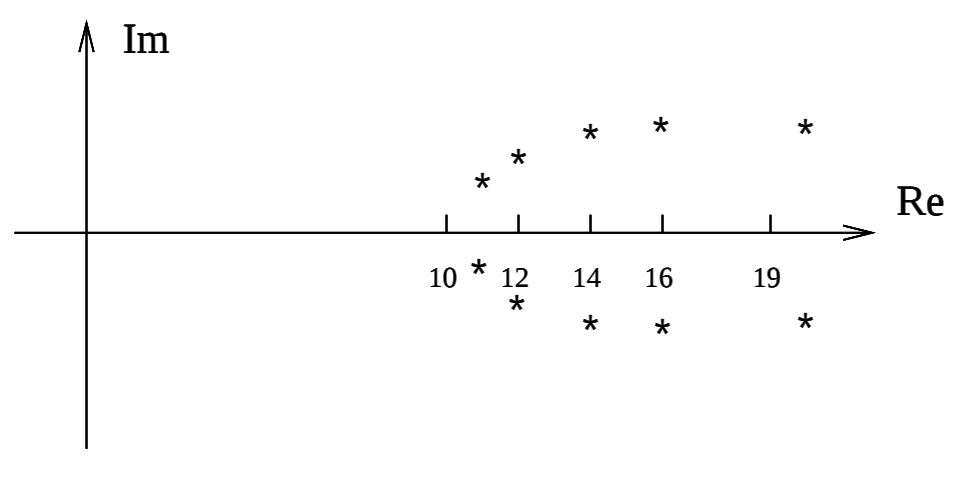
\includegraphics[width=\linewidth]{img/2/2_4_wilkinson_plot}
          \[
              \frac{
                  \partial x
              }{
                  \partial \alpha
              } = \frac{
                  \frac{\partial p}{\partial \alpha}
              }{
                  \frac{\partial p}{\partial x}
              } = \frac{
                  x^{19}
              }{
                  \sum_{i=1}^{20} \prod_{j=1, j \neq i}^{20} (x-j)
              }
          \]
          \[ 
              \left.
                  \frac{\partial x}{\partial \alpha}
              \right|_{x=1} = \frac{
                  i^{19}
              }{
                  \prod_{j=1, j \neq i}^{20}
              }, i = 1, 2, ..., 20
          \]
    	\end{column}
        \begin{column}{.3\linewidth}
          \begin{tabular}{r | l}
              i & $\left.
                  \frac{\partial x}{\partial \alpha}
              \right|_i$ \\
              \hline
               1 & $-8.2 \cdot 10^{-18}$ \\
               2 & $ 8.2 \cdot 10^{-11}$ \\
               5 & $-6.1 \cdot 10^{-1}$  \\
               6 & $ 5.8 \cdot 10^{1}$   \\
               8 & $ 6.0 \cdot 10^{4}$   \\
              10 & $ 7.6 \cdot 10^{6}$   \\
              15 & $-2.1 \cdot 10^{9}$   \\
              19 & $-3.1 \cdot 10^{8}$   \\
              20 & $ 4.3 \cdot 10^{7}$   \\
          \end{tabular}
        \end{column}
    \end{columns}
    \end{exampleblock}
\end{frame}
%%%%%%%%%%%%%%%%